\chapter{Rekurzívne clustrovanie pod dohľadom užívateľa}

Všetky algoritmy zmienené v~predchádzajúcej kapitole pomerne dobre odhaľujú parsovacie vzory, ktoré sa v~danom datasete objavujú často, a ich výsledky sú presné. Aby sme ale dosiahli odhalenie všetkých parsovacích vzorov pri zachovaní vysokej presnosti, musíme sa vysporiadať s~obmedzeniami clustrovacích algoritmov \parencite{Tovarnak2017}.

\subsection*{Rozdelenie správy na tokeny}
Prvým krokom všetkých prezentovaných algoritmov je rozdeliť parsovaciu správu na tokeny. V~tomto smere je potrebná väčšia variabilita pri~zadávaní oddeľovača slov. Nie všetky algoritmy totiž podporujú možnosť zadať aj iný oddeľovač ako medzera, ale ani podpora via\-cerých oddeľovačov tokenov nie je dostačujúca, ako si ukážeme na~príklade. \\

\indent \emph{Starting server with param timeout=2000 ms} \\
\indent \emph{Processing request 127.0.0.1/api/patterns?page-size=10\&page=3} \\

V~prvom prípade chceme použiť ako delimiter aj znak \emph{=} . V~druhom prípade je žiadúce, aby celá url adresa bola zachytená ako jeden para\-meter. Delimiter \emph{=} teda použiť nechceme, a preto by možnosť použiť iný delimiter pre rôzne logovacie správy pomohla ďalej spresniť výsledné parsovacie vzory.

\subsection*{Vstupné parametre}
Hodnota vstupných parametrov je vo vačšine prípadov jedným z~hlav\-ných faktorov, ktorý ovplyvňuje kvalitu výsledných parsovacích vzorov.
Pre~tieto hodnoty existujú odporúčania, ale najpresnejší výsledok získame až po manuálnej analýze datasetu, kde užívateľ po prezre\-tí správ datasetu spustí párkrát daný algoritmus a pokúsi sa nájsť parametre, pre ktoré budú výsledné parsovacie vzory čo najpresnej\-šie.

\subsection*{Kontrola výsledných parsovacích vzorov}
V~závislosti od vyššie zmienených nastavení dostaneme parsovacie vzory, ktoré buď zodpovedajú našej predstave alebo nie. Komplikovanejšia situácia nasáva v~prípade, ak neexistuje všeobecné nastavenie algoritmu, ktoré by vrátilo všetky parsovacie vzory v~potrebnej kvalite. Tento problém sa dá obísť užívateľským rozdelením datasetu na menšie časti a na každú časť pustiť algoritmus s~vlastným nastavením. Toto je ale komplikované, zdĺhavé, náchylne k~chybám a~v~ne\-poslednom rade aj užívateľsky neprívetivé.

\section{RURC -- Recursive User-Reviewed Clustering}
\label{sec:rurc}
Z~hore uvedeného rozboru vyplýva, že ideálny algoritmus by mal zahrňovať určitý stupeň užívateľskej interakcie a mal by vedieť pracovať aj nad vybranou podmnožinou daného datasetu.
\par Vedúci práce, RNDr. Daniel Tovarňák, preto v~\parencite{Tovarnak2017} navrhol syste\-matický postup nazvaný \emph{Recursive User-Reviewed Clustering} znázornený na obr. \ref{fig:rurc}. Výsledkom je proces, pri ktorom užívateľ rekurzívne spúšťa algoritmus nad datasetom, pričom v~každom priebehu má možnosť potvrdiť finálne parsovacie vzory a odfiltrovať z~datasetu správy, ktoré k~nim patria.
\par Tento proces prebieha v~nasledujúcich krokoch:

\begin{enumerate}
  \item Odstránenie správ z~datasetu, ktoré prislúchajú k~už odhaleným parsovacím vzorom.
  \item Úvodný beh algoritmu s~defaultnými parametrami.
  \item Užívateľ rozhodne, ktoré parsovacie vzory sú akceptovateľné, a~tým zároveň z~datasetu odstráni príslušné správy.
  \item Užívateľ buď:
  	\begin{enumerate}
   		 \item spustí algoritmus nad celým datasetom so zmenenými parametrami a pokračuje od bodu 3.
   		 \item označí množinu vzorov, ktoré nie sú vhodné, spustí algoritmus nad podmnožinou datasetu, ktorá prislúcha k~vyb\-raným vzorom, a 				pokračuje od bodu 3.
   		 \item ukončí proces. Proces tiež končí, ak už neostali žiadne správy na spracovanie.
 	 \end{enumerate}
\end{enumerate}

\begin{figure}[htbp]
 \centering 
 \begin{minipage}{\linewidth}
 	\centering
 	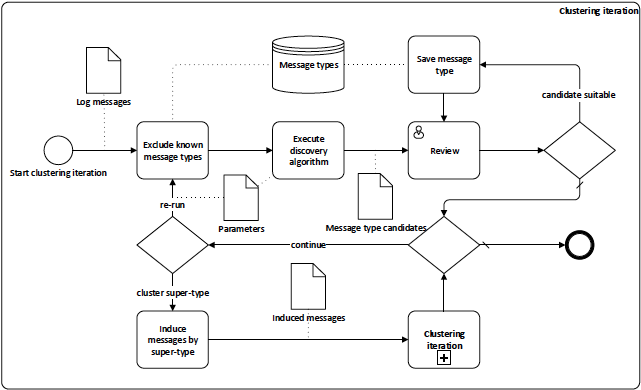
\includegraphics[width=\textwidth]{images/RURC.png} 	
 \end{minipage}
  \caption{Recursive User-Reviewed Clustering, obr. prevzaný z~\parencite{Tovarnak2017}}
  \label{fig:rurc}
\end{figure}


\section{Extended Nagappan-Vouk algoritmus}
\label{sec:eng}
RURC definuje všeobecné princípy analýzy logovacích súborov, avšak nešpecifikuje algoritmus, ktorý má byť použitý na clustrovanie správ.
Z~nedostatkov zmienených v~predchádzajúcej kapitole ale vyplýva, že žiaden algoritmus okrem LogCluster sa nehodí na použitie v~RURC.
\par RNDr. Daniel Tovarňák preto vyvinul algoritmus Extended Na\-gappan-Vouk určený pre použitie v~RURC, ktorý bude spĺnať všetky požiadavky RURC a zároveň bude jednoduchšie nastaviteľný ako LogCluster. Algoritmus produkuje parsovacie vzory vo formáte, ktorý popisuje parameter ako \emph{\%\{m,n\}} $\%\{m,n\}$. Podobne ako pri LogClustry to označuje \emph{m} až \emph{n} za sebou idúcich tokenov. Napr. parsovací vzor \emph{Software caused \%\{1,3\}} zachytí správu ktorá obsahuje text \emph{Software caused} nasledovaný 1 až 3 slovami oddelenými medzerou. \newpage \par Postup algoritmu:

\begin{enumerate}
 \item Správy sa rozdelia na tokeny na základe užívateľom zadaných oddeľovačov slov.
 \item Algoritmus vybuduje frekvenčnú tabuľku rovnako ako pri klasickom Nagappan-Vouk algoritme. Rozdiel je však v~tom, že~algoritmus si ukladá aj pozície rozdeľovačov slov.
 \item Pre každú správu si vo frekvenčnej tabuľke vyhľadáme frekvencie všetkých tokenov správy. Rozdiel oproti Nagappan-Vouk algoritmu je ten, že hraničnú frekvenciu určíme metódou q-per\-centilu poďla užívateľom zadanej vstupnej hodnoty. Podľa toho označíme tokeny ako statickú časť alebo wildcard.
 \item Použitím heuristiky algoritmus skúsi odhaliť prekrývajúce sa clustre a v~prípade, že také clustre existujú, pripojí špecifickejší cluster k~viac všeobecnému.
 \item Algoritmus deteguje po sebe idúce sekvencie wildcard v~doposiaľ nájdených vzoroch a ak je to možné, tieto sekvencie spojí a~vytvorí
 vzor s~dolnou a hornou hranicou spojených tokenov.
\end{enumerate}

\subsection{Data mining}
\label{sec:data-mining}
Ako sme spomenuli v~sekcii \ref{sec:eng}, Extended Nagappan-Vouk produkuje parametre vzoru vo formáte \emph{\%\{m,n\}}. Výsledný parsovací vzor je teda kompaktný a užívateľsky čitateľný.  Tento formát vieme ďalej jednoduchou úpravou previesť na regulárny výraz, používaný štandardnými knižnicami.
\par Po odhalení všetkých parsovacích vzorov, väčšinou príde na rad data mining, tzn. pre každú logovaciu správu extrahujeme parametre jej parsovacieho vzoru. To vykonáme nájdením jej parsovacieho vzoru a vrátením zachytených skupín regulárneho výrazu. Triviálny, ale často používaný postup je iterovať cez všetky vzory až kým sa nenájde zhoda. V~najhoršom prípade to znamená prejsť celú množinu vzorov. Takýto prístup je ale neefektívny a môže spôsobovať výkonnostné problémy.
\par Kvôli odstráneniu vyššie zmienených problémov, RNDr. Daniel Tovarňák v~\parencite{regextrie} navrhol stromovú štruktúru Regex Trie - REtrie a~algoritmus, ktorý v~danej štuktúre nájde príslušný parsovací vzor so~zložitosťou $\mathcal{O}(t)$, kde $t$ je počet tokenov v~správe.
\par REtrie akceptuje parsovacie vzory vo formáte YAML súboru:

\begin{figure}[h]
\centering
\begin{minipage}{\textwidth}
\lstset{columns=flexible,breaklines=true,breakatwhitespace=true, showstringspaces=false}
\begin{lstlisting}
regexps:
  INT: [integer, '[0-9]+']
  STRING: [string, '[!-~]+']
  
patterns:
  default:
    pattern1:'Generating %{INT:var1} bit RSA key'
  ssh:
   pattern1:'Illegal user %{STRING:var1} from %{STRING:var2}'
\end{lstlisting} 		
\end{minipage} 
\end{figure}

Pod kľúčom regexps je zoradený zoznam typov regulárnych výrazov. Každý takýto typ sa skladá z~mena, dátového typu a samotného regulárneho výrazu. Kľúč patterns obsahuje parsovacie vzory, ktoré sú združené pod ľubovoľným identifikátorom skupiny vzorov. Parameter parsovacieho vzoru sa potom skladá z~odkazu na typ regulárneho výrazu a mena. Pri hľadaní vhodného typu sa postupuje zhora nadol a použije sa prvý vhodný typ, ktorý sa nájde. Preto je dôležité poradie v~ako sú dané typy uvedené.  Aby sme mohli ťažiť z~tohto prístupu, výsledný systém musí vedieť zvládnuť konverziu medzi prezentovanými formátmi parsovacích vzorov.